\documentclass{beamer}
% compress?
\usepackage[utf8]{inputenc}
\usepackage[T1]{fontenc}

\usepackage{varwidth}
\usepackage{caption}
\usepackage{xcolor}
\usepackage{tikz,pgfplots}
\pgfplotsset{compat=1.18}
\usepackage{subcaption}
\usepackage{graphicx}
\usepackage{listings}
\usepackage{comment}


\usetheme{Dresden}
\useoutertheme[footline=authorinstitutetitle,subsection=false]{miniframes}

% \definecolor{ThemeColor}{rgb}{200/255, 69/255, 147/255}
\definecolor{ThemeColor}{rgb}{0.7, 0.5, 0.0}
\usecolortheme[named=ThemeColor]{structure}

% \setbeamertemplate{footline}[frame number]
% \setbeamertemplate{footline}{
    % \begin{beamercolorbox}[right]{author in head/foot}%
        % \insertframenumber{} / \inserttotalframenumber
    % \end{beamercolorbox}%
% }

\AtBeginSection[]{
    \begin{frame}
    \vfill \centering
    \begin{beamercolorbox}[sep=8pt, center, shadow=true, rounded=true]{title}
        \usebeamerfont{title}\insertsectionhead\par%
    \end{beamercolorbox}
    \vfill
    \end{frame}
}



\title{A Theoretical Model for Lexicon Entropy in Emergent Language}
\author{Brendon Boldt, David Mortensen}
\date{\today}
% \addtobeamertemplate{navigation symbols}{}{\quad\includegraphics[width=2em]{ih-white}}
\addtobeamertemplate{navigation symbols}{}{\hspace{0.2em}\rm \raise1ex\hbox{JM\raise 1ex\hbox{\kern-0.7em\textdagger}\kern0.1emJ}}
% \addtobeamertemplate{navigation symbols}{}{\quad M\raise 1ex\hbox{\kern-0.7em\textdagger}\kern -0.75em\raise 0.5ex\hbox{---}}
% JM\raise 1ex\hbox{\kern-0.7em\textdagger}\kern0.25emJ
% M\raise 1ex\hbox{\kern-0.7em\textdagger}\kern -0.75em\raise 0.5ex\hbox{---}


\renewcommand{\thesubfigure}{\arabic{figure}.\alph{subfigure}}

\newif\ifusevizzes
% \usevizzestrue
\usevizzesfalse


\begin{document}

\maketitle

% TODO
% Rehearse entropy tradeoff speech
% Make slide introducing model
% Talk about environment hyperparameters when first introduced?
% Remove caveat

%%% Presentation Times %%%
% Overview       1:30
% Background     6:30
% The Model     16:30
% Experiments    6:15
% Sig of Models  9:30
% Review         1:05
% Total         41:20

\begin{comment}

\section{Overview}

\begin{frame}{This talk}
    \begin{itemize}
        \item Introduce an emergent language environment
            \begin{itemize}
                \item And a property we want to measure
            \end{itemize}
        \item Define a mathematical model of this property
        \item Compare the model's predictions to the actual system
        \item Discuss models and their role more generally
    \end{itemize}
\end{frame}

\section{Background}

\begin{frame}{Emergent language}
    \begin{enumerate}
        \item Start with a multi-agent reinforcement learning environment
            \begin{itemize}
                \item Agents have communication channel
            \end{itemize}
        \item See how agents learn to interact and communicate
        \item Study the resulting communication protocol
        \item Apply these findings
    \end{enumerate}
\end{frame}

\begin{frame}{Environment and agent architecture} \begin{center}
    \begin{figure}
        \begin{subfigure}{0.45\linewidth}
            \includegraphics[height=1.2in]{assets/navigation.pdf}
            \caption{Environment}
        \end{subfigure}
        \hfill
        \begin{subfigure}{0.45\linewidth}
            \includegraphics[height=1.2in]{assets/agent-architecture.pdf}
            \caption{Agent architecture}
        \end{subfigure}
    \end{figure}
    \end{center}
\end{frame}

\begin{frame}{Entropy}
    \begin{itemize}
        \item Shannon entropy (from information theory)
            \begin{itemize}
                \item Measures average amount of information per message
            \end{itemize}
        \item Entropy $\approx$ evenness of message distribution
            \begin{itemize}
                \item High entropy $\rightarrow$ close to uniform
                \item Low entropy $\rightarrow$ highly concentrated probability
            \end{itemize}
        \item Fundamental property of communication
            \begin{itemize}
                \item Precision--effort tradeoff
            \end{itemize}
    \end{itemize}
\end{frame}


\section{The Model}

\begin{frame}{Chinese restaurant process}
    \begin{itemize}
        \item Self-reinforcing stochastic process
        \item Yields a distribution over the positive integers
        \item Start with an infinite number of tables
            \begin{itemize}
                \item When a person walks in, sit a table randomly
                    \begin{itemize}
                        \item Probability proportional to \# of people at table
                        \item Sit at new table as if it already had $\alpha$ people
                    \end{itemize}
                \item Repeat
            \end{itemize}
    \end{itemize}
\end{frame}


\begin{frame}{Chinese restaurant process visualization}
    \begin{center}
        \ifusevizzes
            
\begin{tikzpicture}
  \begin{axis}[
    ybar stacked,
    % ybar interval=0.7,
    % grid=x,
    width=9cm, height=6cm,
    xtick=data,
    ytick distance=2,
    ymajorgrids=true,
    yminorgrids=true,
    minor y tick num=1,
    ymin=0,
    ymax=10,
    axis on top,
    grid style={draw=white,line width=0.5mm},
    ]
\only<1>{\addplot[draw=blue,fill=blue] coordinates {(0,0)};}
\only<1>{\addplot[draw=green,fill=green] coordinates {(0, 2)};}
\only<2>{\addplot[draw=blue,fill=blue] coordinates {(0,1)(1,0)};}
\only<2>{\addplot[draw=green,fill=green] coordinates {(0, 0)(1, 2)};}
\only<3>{\addplot[draw=blue,fill=blue] coordinates {(0,1)(1,1)(2,0)};}
\only<3>{\addplot[draw=green,fill=green] coordinates {(0, 0)(1, 0)(2, 2)};}
\only<4>{\addplot[draw=blue,fill=blue] coordinates {(0,1)(1,1)(2,1)(3,0)};}
\only<4>{\addplot[draw=green,fill=green] coordinates {(0, 0)(1, 0)(2, 0)(3, 2)};}
\only<5>{\addplot[draw=blue,fill=blue] coordinates {(0,1)(1,1)(2,2)(3,0)};}
\only<5>{\addplot[draw=green,fill=green] coordinates {(0, 0)(1, 0)(2, 0)(3, 2)};}
\only<6>{\addplot[draw=blue,fill=blue] coordinates {(0,1)(1,1)(2,2)(3,1)(4,0)};}
\only<6>{\addplot[draw=green,fill=green] coordinates {(0, 0)(1, 0)(2, 0)(3, 0)(4, 2)};}
\only<7>{\addplot[draw=blue,fill=blue] coordinates {(0,1)(1,1)(2,3)(3,1)(4,0)};}
\only<7>{\addplot[draw=green,fill=green] coordinates {(0, 0)(1, 0)(2, 0)(3, 0)(4, 2)};}
\only<8>{\addplot[draw=blue,fill=blue] coordinates {(0,1)(1,1)(2,4)(3,1)(4,0)};}
\only<8>{\addplot[draw=green,fill=green] coordinates {(0, 0)(1, 0)(2, 0)(3, 0)(4, 2)};}
\only<9>{\addplot[draw=blue,fill=blue] coordinates {(0,1)(1,1)(2,5)(3,1)(4,0)};}
\only<9>{\addplot[draw=green,fill=green] coordinates {(0, 0)(1, 0)(2, 0)(3, 0)(4, 2)};}
\only<10>{\addplot[draw=blue,fill=blue] coordinates {(0,1)(1,1)(2,5)(3,1)(4,1)(5,0)};}
\only<10>{\addplot[draw=green,fill=green] coordinates {(0, 0)(1, 0)(2, 0)(3, 0)(4, 0)(5, 2)};}
\only<11>{\addplot[draw=blue,fill=blue] coordinates {(0,1)(1,1)(2,5)(3,1)(4,1)(5,1)(6,0)};}
\only<11>{\addplot[draw=green,fill=green] coordinates {(0, 0)(1, 0)(2, 0)(3, 0)(4, 0)(5, 0)(6, 2)};}

  \end{axis}
\end{tikzpicture}

        \else
            \includegraphics[width=7cm]{example-image-a.png}
        \fi
    \end{center}
\end{frame}


\begin{frame}{The analogy}
    \begin{itemize}
        \item Three-way analogy
            \begin{itemize}
                \item Mathematical model
                \item Neural network/RL system
                \item Human language
            \end{itemize}
        \item Tables $\cong$ words
        \item Table population $\cong$ likelihood of using that word
        \item Intuition:
        \begin{itemize}
            \item Used words are learned more
            \item Learned words are used more
        \end{itemize}
    \end{itemize}
\end{frame}

\begin{frame}{\textsc{FiLex}}
    \begin{itemize}
        \item \textbf{Fi}nite \textbf{Lex}icon Stochastic Process
        \item Modification of the Chinese restaurant process
            \begin{itemize}
                \item Finite lexicon
                \item Start with uniform weights
                \item Smooth updates
            \end{itemize}
        \item Analogy with neural network
            \begin{itemize}
                \item Size of update $\cong$ learning rate
                \item \# of tables $\cong$ bottleneck size
                \item \# of steps $\cong$ training steps
            \end{itemize}
    \end{itemize}
\end{frame}

\begin{frame}{\textsc{FiLex} visualization}
    \begin{center}
    \ifusevizzes
          
\begin{tikzpicture}
  \begin{axis}[
    ybar stacked,
    % ybar interval=0.7,
    % grid=x,
    width=9cm, height=6cm,
    xtick=data,
    ytick distance=2,
    ymajorgrids=true,
    yminorgrids=true,
    minor y tick num=1,
    ymin=0,
    ymax=10,
    axis on top,
    grid style={draw=white,line width=0.5mm},
    ]
\only<1->{\addplot[draw=green,fill=green] coordinates {(0,1)(1,1)(2,1)(3,1)(4,1)};}
\only<2>{\addplot[draw=blue,fill=blue] coordinates {(0, 0)(1, 0)(2, 0)(3, 0)(4, 1)};}
\only<3>{\addplot[draw=blue,fill=blue] coordinates {(0, 0)(1, 0)(2, 0)(3, 1)(4, 1)};}
\only<4>{\addplot[draw=blue,fill=blue] coordinates {(0, 0)(1, 0)(2, 0)(3, 2)(4, 1)};}
\only<5>{\addplot[draw=blue,fill=blue] coordinates {(0, 0)(1, 0)(2, 0)(3, 3)(4, 1)};}
\only<6>{\addplot[draw=blue,fill=blue] coordinates {(0, 1)(1, 0)(2, 0)(3, 3)(4, 1)};}
\only<7>{\addplot[draw=blue,fill=blue] coordinates {(0, 1)(1, 0)(2, 0)(3, 4)(4, 1)};}
\only<8>{\addplot[draw=blue,fill=blue] coordinates {(0, 1)(1, 0)(2, 0)(3, 5)(4, 1)};}
\only<9>{\addplot[draw=blue,fill=blue] coordinates {(0, 1)(1, 0)(2, 0)(3, 6)(4, 1)};}
\only<10>{\addplot[draw=blue,fill=blue] coordinates {(0, 1)(1, 0)(2, 0)(3, 7)(4, 1)};}
\only<11>{\addplot[draw=blue,fill=blue] coordinates {(0, 1)(1, 0)(2, 1)(3, 7)(4, 1)};}
\only<12>{\addplot[draw=blue,fill=blue] coordinates {(0, 1)(1, 0)(2, 1)(3, 7)(4, 2)};}

  \end{axis}
\end{tikzpicture}

      \else
          \includegraphics[width=7cm]{example-image-b.png}
      \fi
    \end{center}
\end{frame}

\section{Experiments}

\begin{frame}{Experiments}
    \begin{itemize}
        \item Compare hyperparameter sweeps with the model and system
        \item Model parameters adjusted to imitate system
            \begin{itemize}
                \item Correspondence between HPs not $1:1$
            \end{itemize}
        \item Primarily qualitative, looking at general trends
    \end{itemize}
\end{frame}

\begin{frame}{Plot comparison}
    \begin{center}
        \begin{figure}
            \def\plotheight{0.8in}
            \def\subfigwidth{0.30}
            \centering

            \begin{subfigure}[t]{0.36\linewidth}
                \centering
                \rotatebox{70}{\scriptsize\hspace{2em}FiLex}
                \includegraphics[height=\plotheight]{assets/model-alpha.pdf}
                % \caption{\theProcess\@: $1/\alpha$}\label{fig:beta}
                \hbox{
                    \rotatebox{70}{\scriptsize\hspace{2em}System}
                    \hspace{0.1em}
                    \includegraphics[height=\plotheight]{assets/learning_rate_log-entropy-default.pdf}
                }
                \caption{\scriptsize learning rate}
            \end{subfigure}
            % \begin{subfigure}[t]{\subfigwidth\linewidth}
            %     \centering
            %     \includegraphics[height=\plotheight]{assets/model-beta.pdf}
            %     % \caption{\theProcess: $\beta$}\label{fig:beta}
            %     \includegraphics[height=\plotheight]{assets/n_steps_log-entropy-default.pdf}
            %     \caption{$\beta$ and rollout buffer size}
            % \end{subfigure}
            \begin{subfigure}[t]{\subfigwidth\linewidth}
                \centering
                \includegraphics[height=\plotheight]{assets/model-n_params.pdf}
                % \caption{\theProcess: \texttt{n\_params} }\label{fig:beta}
                \hbox{
                    \hspace{-0.0em}
                    \includegraphics[height=\plotheight]{assets/bottleneck_size_log-entropy-default.pdf}
                }
                \caption{\scriptsize bottleneck size}
            \end{subfigure}
            \begin{subfigure}[t]{\subfigwidth\linewidth}
                \includegraphics[height=\plotheight]{assets/model-n_iters.pdf}
                % \caption{\theProcess: \texttt{n\_iters}}\label{fig:beta}
                % \centering
                \hbox{
                    \hspace{-0.15em}
                    \includegraphics[height=\plotheight]{assets/total_timesteps_log-entropy-default.pdf}
                }
                \caption{\scriptsize training steps}
            \end{subfigure}

            % \caption{
            %     Plots for entropy vs.\@ various hyperparameters.
            %     \theProcess{} is plotted in orange and the ELS in blue.
            % }\label{fig:plots}
        \end{figure}
    \end{center}
\end{frame}

\begin{frame}{Discussion}
    \begin{itemize}
        \item Model and system have functional similarities
            \begin{itemize}
                \item Conceptually, by analogy
                \item Experimentally
            \end{itemize}
        \item Reasoning with the model applies to system
            \begin{itemize}
                \item Explanation
                \item Prediction
            \end{itemize}
    \end{itemize}
\end{frame}

\section{Significance of Models}
\end{comment}

%%% TODO bold things as needed

% model matches system
% models are used for explanation and prediction

% model yield experiments
% implicit and explicit models
% explicit models are easier to express
% experiments reflect on models; theory building

\begin{frame}{Why are models important?}
    \begin{itemize}
        \item Explanation
        \item Prediction
        \item How we communicate concepts
        \item All experiments are based on models
    \end{itemize}
\end{frame}

\begin{frame}{The role of models}
    \begin{itemize}
        \item Experiments have a \emph{raison d'\^etre}
        \item This reasoning comes from models
        \item Two kinds of models:
            \begin{itemize}
                \item \textit{Explicit:} mathematical, precise
                \item \textit{Implicit:} intuition, analogy
            \end{itemize}
        \item This paper illustrates an explicit model
    \end{itemize}
\end{frame}

\begin{frame}{Advantage of explicit models}
    \begin{itemize}
        \item What happens when the model is proved wrong?
            \begin{itemize}
                \item \textit{Explicit:} revise, improve
                \item \textit{Implicit:} change intuitions, I guess\ldots
            \end{itemize}
        \item Mathematical models go beyond initial assumptions
        \item Explicit models are easier to express
            \begin{itemize}
                \item But difficult to apply to deep learning
                \item Seldom used in applications
            \end{itemize}
        % \item \emph{Negative results can be interesting!}
    \end{itemize}
\end{frame}

\begin{frame}{Future work}
    \begin{itemize}
        \item Rigorous analysis of empirical results
        \item Form a clear hypothesis
            \begin{itemize}
                \item Must be falsifiable (able to be refuted based on evidence)
                \item e.g., statistical significance criteria
            \end{itemize}
        \item Allows us to demonstrate:
            \begin{itemize}
                \item Where there is evidence for the model
                \item Where the model does not work
                \item Determine what would fix the model
            \end{itemize}
    \end{itemize}
\end{frame}

\begin{frame}{Review}
    \begin{enumerate}
        \item Illustrate what an explicit model looks like
            \begin{itemize}
                \item Specifically for a deep learning-based field
            \end{itemize}
        \item Argue for the importance of explicit models
    \end{enumerate}
\end{frame}

\end{document}
